\subsection{Initial object analysis}
The table describes the predicted classes and their purpose and relations. This will be elaborated on when the class diagram will be added in assignment 38.
\\
\HRule \\[0.4cm]
\emph{Event}\\
A collection of information such as DATE, TIME, DESCRIPTION, NOTIFICATION, TAG.\\
\HRule \\[0.4cm]
\emph{Calendar}\\
Holds an abitrary number of EVENTS\\
\HRule \\[0.4cm]
\emph{User}\\
A person who uses the system, who wants to get an overview of the events he/she has.\\
\HRule \\[0.4cm]
\emph{PAC-CLOUD}\\
A storage unit who can send and retrieve CALENDARs for USERs\\
\HRule \\[0.4cm]
\emph{Notification}\\
A message prompting the USER with information about an upcoming EVENT\\
\HRule \\[0.4cm]
\emph{Tag}\\
An one-worded description of an EVENT - used to group simular kinds of events together.\\
\HRule \\[0.4cm]
\emph{Notifier}\\
A collection of notifications that will be popped and shown to the user when a time threshold has been exceeded.\\
\HRule \\[0.4cm]
\emph{View}\\
A visual representation of the CALENDAR to the USER\\
\HRule \\[0.4cm]

\textbf{Analysis Object Model (Static Model):}\\
This table contains our Entity, Control and Boundry objects, that are being used in our system, at the moment.
These objects are being used to make our class diagram\\
\\
\begin{tabular}{l | l | l}

Entity    	& Control 			& Boundry 		\\
\toprule
Event     	& CreateCalendarEntry	& CalendarView	\\
Calendar	& UpdateCalendarEntry	& EventView 		\\
User		& ChangeOverviewType	& NoticeView		\\
Notification	& ChooseTag			& LoginView		\\
Tag		& CreateTag			&			\\
		& SetNotification		&			\\
		& GetNotification		&			\\		
		& CreateHistoryReport	&			\\
		& CancelEntry		&			\\
		& Login			&			\\		
		
\bottomrule
\end{tabular}\\
\\

This is our class diagram. All our Entity, Control and Boundry objects are represented in our class diagram, 
and our class diagram shows how our objects are connected to each other.\\
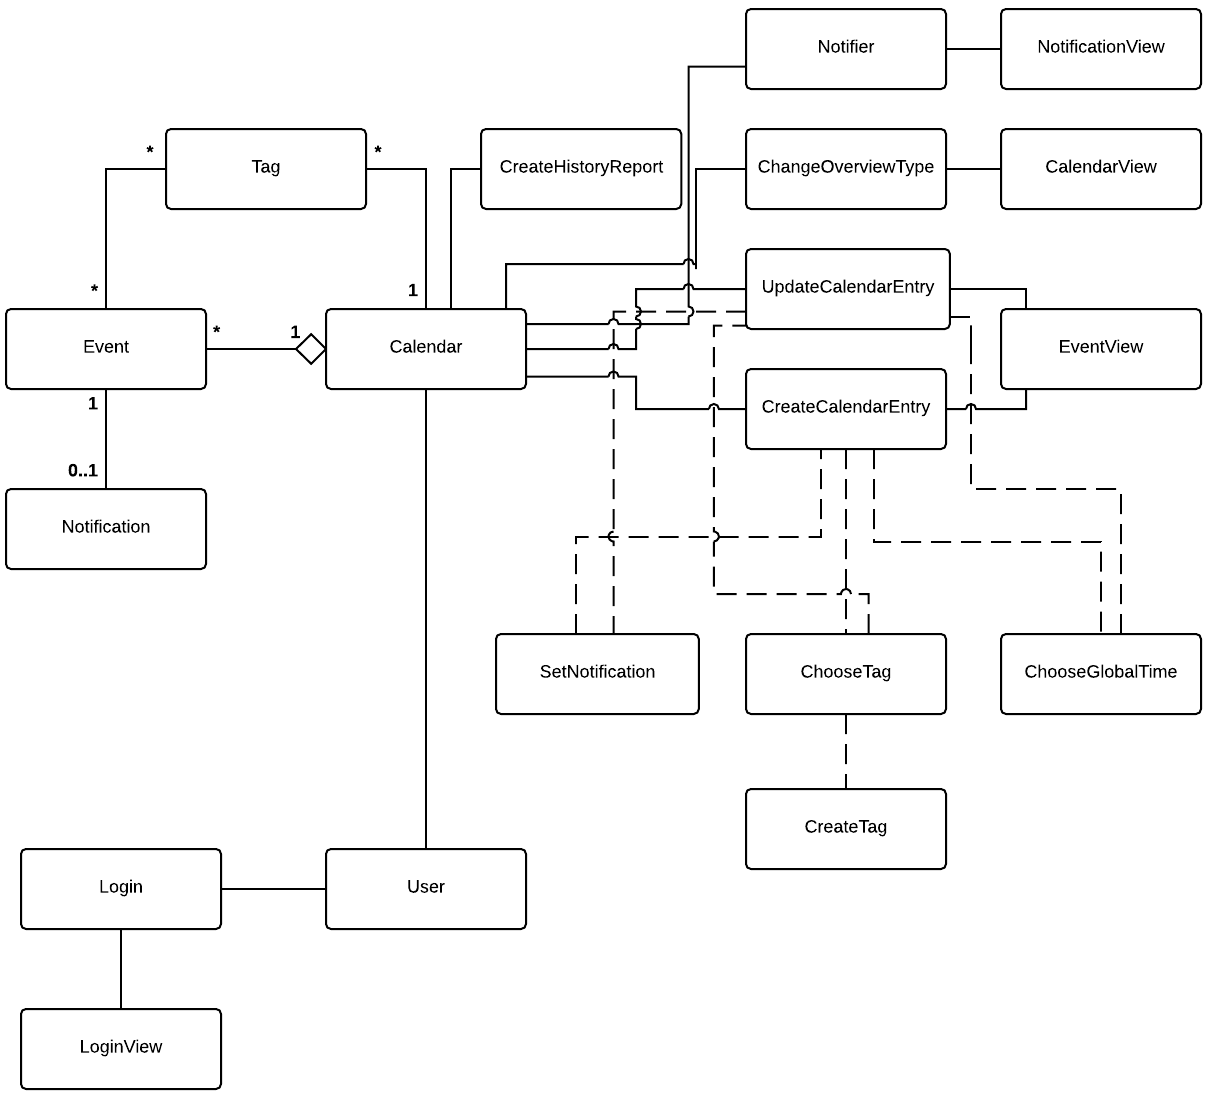
\includegraphics[scale=0.4]{UMLClassDiagram}